%Following is an open list of problems that we will address in order to achieve device composition by means of implicit interaction.
%\begin{enumerate}
%\item{\emph{Setup}: How is a device enabled for integrating with a tabletop?
%The setup should be simple, to be performed only once by non-technical users.
%An initial survey of possible solutions points towards the use of tagging mechanisms and/or camera-based object recognition.}
%\item{\emph{Discovery}: How do the tabletop and the device discover and communicate with each other?
%How do we solve the issues of discovery, handshake, network connectivity, and encryption mechanisms to ensure privacy?}
%\item{\emph{UI transfer}: Given the computational constraints of mobile devices, how can the UI transfer be efficiently implemented so as to support native applications and guarantee a seamless user experience?}
%\item{\emph{Input}: How can the users interact with their applications on the tabletop (touch and other peripherals)?}
%\item{\emph{Interaction Design}: What means of interaction are best-fitted for the tabletop-based systems that we propose to develop?
%How can we best adapt to public/private uses and single/multiple users?
%How can we take advantage of the larger interaction surface?}
%\end{enumerate}

%%%%%%%%%%%%%%%%%%%%%%
%%% IMPLEMENTATION %%%
%%%%%%%%%%%%%%%%%%%%%%

\chapter{The TIDE prototype}
\label{system}

TIDE (Tabletop Interactive Display Extension) is a composite device between smartphones and a tabletop computer.
It replicates the smartphone's user interface on the tabletop, where it can be manipulated and interacted with.
The application can handle simultaneous devices.
%that integrates smartphones to a tabletop by way of UI replication.
It runs on the Microsoft Surface tabletop computer, referred to as \emph{Surface} in this chapter.
It currently supports two smartphone models: the iPhone 4 (iOS 5) and the HTC Legend (Google Android 2.1), and can be extended to support other models.

\begin{figure}[htb]
  \centering
    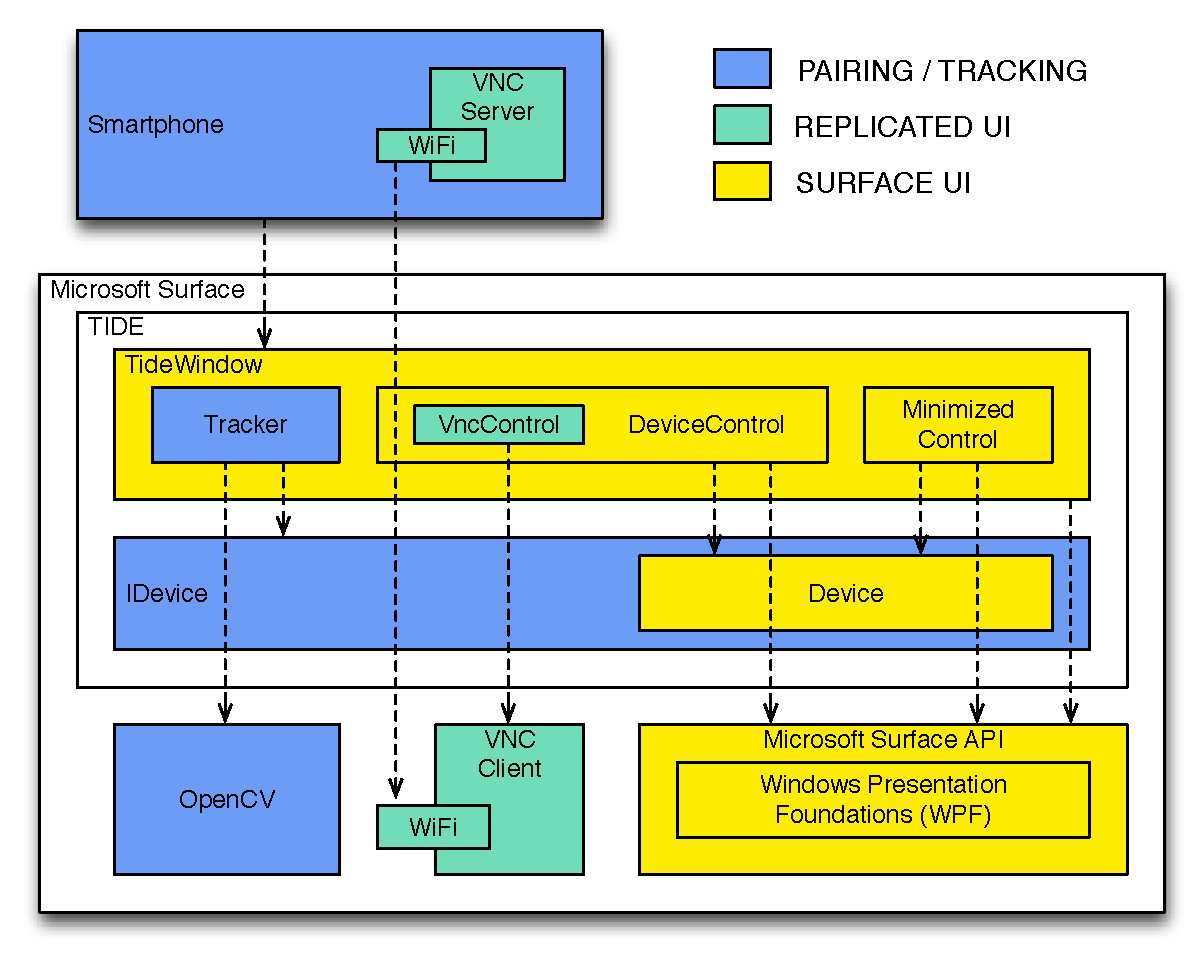
\includegraphics[width=0.8\textwidth]{images/overviewNew}
    \caption{TIDE component diagram.}
    \label{fig:overview}
\end{figure}

Figure~\ref{fig:overview} is a component diagram that presents an overview of the system.
TIDE can be divided into three parts, which together implement the design aspects formulated in section~\ref{sec:design}, i.e.\ pairing, tracking, replicated UI and surface UI.

The pairing and tracking elements (blue) are presented in sections \ref{sec:pairing} and \ref{sec:tracking}.
They are both based on shape recognition in order to detect the presence and location of the smartphone on the tabletop.
To do that, TIDE uses the visual input provided by the Surface camera, and otherwise relies on OpenCV (Open Source Computer Vision) \citeyearpar{opencv}, a library that provides the tools necessary to process images and perform object detection.

Replicating the smartphone's UI (green) is described in section~\ref{sec:replicatedui}.
It is done with VNC \citep{Richardson:1998:vnc}, a platform-independent system for standard desktop sharing.
TIDE includes a VNC client that is based on the VncSharp library \citep{vncsharp}, and that connects over a WiFi connection to a VNC server running on the smartphone.

Section~\ref{sec:surfaceui} presents the surface UI (yellow).
It was implemented within the .NET framework, using the Surface SDK and WPF (Windows Presentation Foundations).
It links the other components together in a Surface application, and provides the overall user interface.
The surface UI is the system aspect that has the most relevance for the user interaction, and therefore has received most focus in this implementation.

\section{System interaction}

Using the system involve a user, a smartphone and a tabletop computer interacting with each other.
During a typical session, the interaction revolves around the \emph{surface UI}, which is the interface between all system parts, and is contained by the main application window on the tabletop, the \texttt{TideWindow}.
Figure~\ref{fig:sequenceOverview} is a sequence diagram that describes this interaction.

The \emph{user} starts the session by placing the smartphone on the table (\raisebox{.5pt}{\textcircled{\raisebox{-.9pt} {1}}}), where it is detected by the \emph{tracker} component (\raisebox{.5pt}{\textcircled{\raisebox{-.9pt} {2}}}).
Optionally, the tracker can track the device during the whole application session.
Upon device detection, a virtual device is created and added to the surface UI, then forwarded to the \emph{VNC client} which is responsible for establishing the connection (\raisebox{.5pt}{\textcircled{\raisebox{-.9pt} {3}}}).
The VNC client attempts to connect to the \emph{VNC server} running on the smartphone (\raisebox{.5pt}{\textcircled{\raisebox{-.9pt} {4}}}), at which point an explicit authorization from the user is required.
If the connection is authorized, the server sends the smartphone UI to the client for replication.

At this point, the session enters a \emph{loop} where the user interacts with the surface UI for an undefined amount of time.
The user provides input to the surface UI, a part of which is destined for the replicated UI.
The VNC client sends the said input to the server, which responds with a new copy of the smartphone screen, that is used by the surface UI to update the replicated UI.

On the initiative of the user, the session is terminated, at which point the virtual device is removed from the \texttt{TideWindow}, and the connection is interrupted by the VNC client.

\begin{figure}[htb]
  \centering
    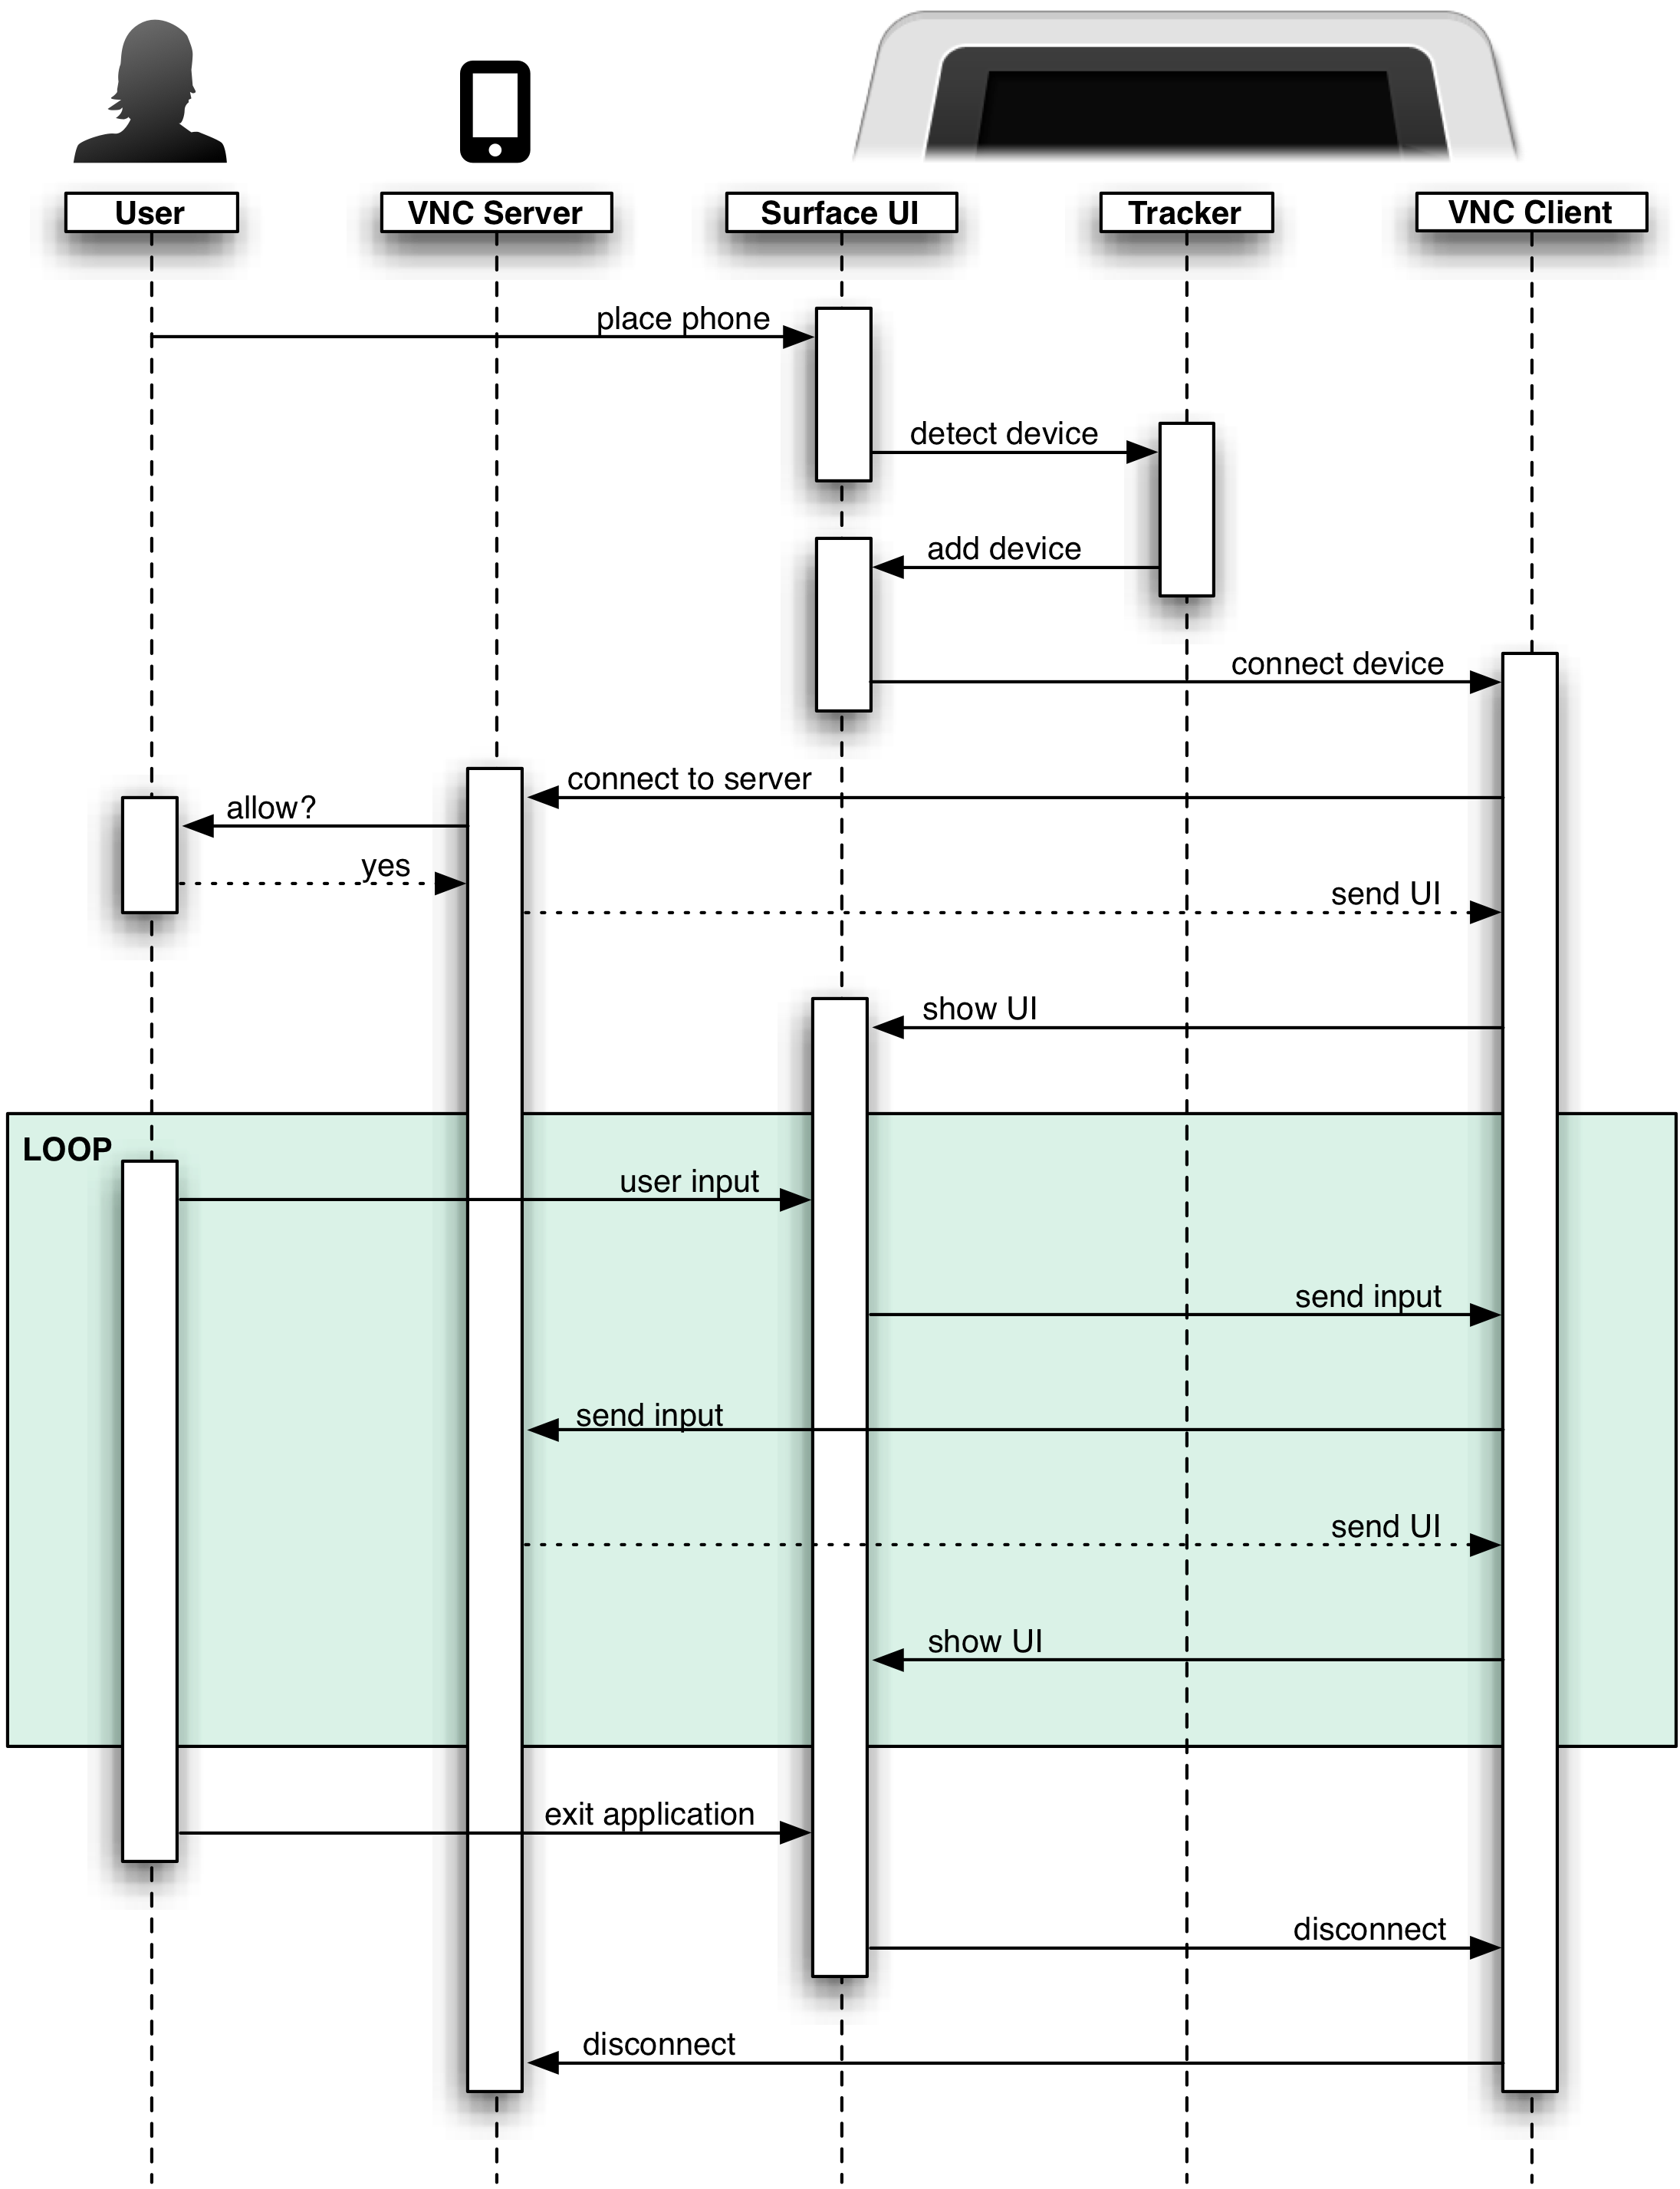
\includegraphics[width=0.8\textwidth]{images/sequenceOverview}
    \caption{TIDE: main interaction diagram.}
    \label{fig:sequenceOverview}
\end{figure}


%\clearpage

%%%%%%%%%%%%%%
%% PAIRING %%
%%%%%%%%%%%%%%
\section{Pairing}
\label{sec:pairing}

This section describes and explains the implementation steps that were taken based on the design decisions in section~\ref{sec:design} relating to the pairing procedure.

%In the case of the smartphone, this connection is very likely wireless.
%Moreover, a VNC server instance should be up and running on the smartphone, for the system to function.

The pairing procedure consists of three steps
(1) A \emph{trigger} starts the procedure
(2) \emph{Discovery} allows the smartphone's local IP address to be made available to the tabletop
(3) The \emph{connection} is established, given that the user explicitly authorizes it.

\subsection{Trigger}

To realize the design decision
\emph{DA-1a Pairing is triggered by placing the smartphone on the tabletop},
TIDE uses the Surface computer vision to detect when a smartphone is placed on the tabletop.

The implementation details of the smartphone detection and tracking are presented in section~\ref{sec:tracking}.

\subsection{Discovery}

For the tabletop to discover the local IP address of the smartphone, a straightforward solution is to present a text field to the user in which s/he can enter it.
However, this approach has several limitations, including an obvious lack of spontaneity.
Not all smartphone users know where to look in the device's settings to find the IP address, and in any case, it is a process of several steps that hinders the spontaneity, which is the overall aim of this prototype.

Therefore, to realize the design decision
\emph{DA-2 Device discovery relies on a standard networking protocol},
TIDE should use an automatized discovery process, based on a standard networking protocol, such as the ones provided by UPnP \citep{upnp} and Bonjour \citep{bonjour}.

However, given that the focus of this thesis lies on the user interaction problem, 
%is not to contribute within this area,
% and for reasons of time constraints, 
it was decided not to implement the discovery protocol.
The system currently functions with IP addresses hardcoded into the TIDE implementation on the Surface, to serve the purpose of the proof-of-concept.

\subsection{Connection}

The design decision
\emph{DA-1b Pairing is based on wireless connectivity},
does not require any implementation effort, but represents an assumption about device and environment.
There must be a local area network for the system to function, and both devices must be connected to it.
The tabletop being in a fixed location, it can use either WiFi or an ethernet cable.
On the smartphone, WiFi must be used.

To realize the design decision
\emph{DA-3 The user must confirm the connection, both on the tabletop and on the smartphone},
TIDE uses dialogs, that appear successively on the tabletop, then on the smartphone.
They are described further in section~\ref{sec:surfaceui}.

%\clearpage
%%%%%%%%%%%%%%
%% TRACKING %%
%%%%%%%%%%%%%%
\section{Tracking}
\label{sec:tracking}

This section describes and explains the implementation steps that were taken based on the design decisions in section~\ref{sec:design} relating to tracking the location of smartphones on the tabletop.
To realize the design decisions DB-1 to DB-3 (see p.~\pageref{DB}), TIDE uses the computer vision provided by the Surface, as well as the OpenCV library.

The Surface uses camera-based vision to detect touch input.
Infrared light is projected towards the surface, and reflected by the objects that are in contact with the table.
This reflection is captured by infrared cameras, allowing the Surface to ``see'' all types of shapes.
When such a shape is small enough, the Surface interprets it as a finger, and reacts accordingly.

Beside fingers, the Surface is designed to natively recognize certain types of 2D visual tags (Byte and Identity tags).
Such tags can be used to integrate objects to Surface applications.

However, using visual tags in the present case would imply that the system is only usable to users who have applied such a tag to the smartphone.
To remove as many constraints as possible, and to make the system usable in as many situations as possible, it was decided to use shape recognition.

OpenCV provides algorithms to perform shape analysis and recognition on the raw images that are captured by the Surface system. 
%Thus, specific visual features can be recognized, and 

%By using OpenCV, it is possible to analyze the captured images to detect specific shapes and interpret the nature of the object on the table.

\begin{figure}[htbp]
  \centering
    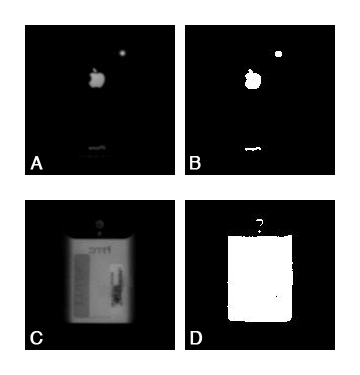
\includegraphics[width=0.5\textwidth]{images/msRaw}
    \caption{Microsoft Surface raw visual input: (A) iPhone 4 (B) iPhone 4 after threshold processing (C) HTC Legend (D) HTC Legend after threshold processing.}
    \label{fig:msRaw}
\end{figure}

Figure~\ref{fig:msRaw} shows the raw Surface input for both smartphones.
The features that allow TIDE to detect the iPhone 4 are the Apple logo and the camera point in the back of the casing.
For the HTC Legend, the system looks for the larger silver rectangle formed by the aluminum casing.

Two things can be remarked on.
First, black casing areas do not reflect infrared light, which is a basic, yet serious limitation, given that certain models of smartphones could be invisible to the system.
Second, detecting a phone depends on the specific features that the phone presents on its casing.
This implies that the system must take into considerations that the phone could be placed on the table face down, or wear a protective sleeve.

\begin{figure}[htbp]
  \centering
    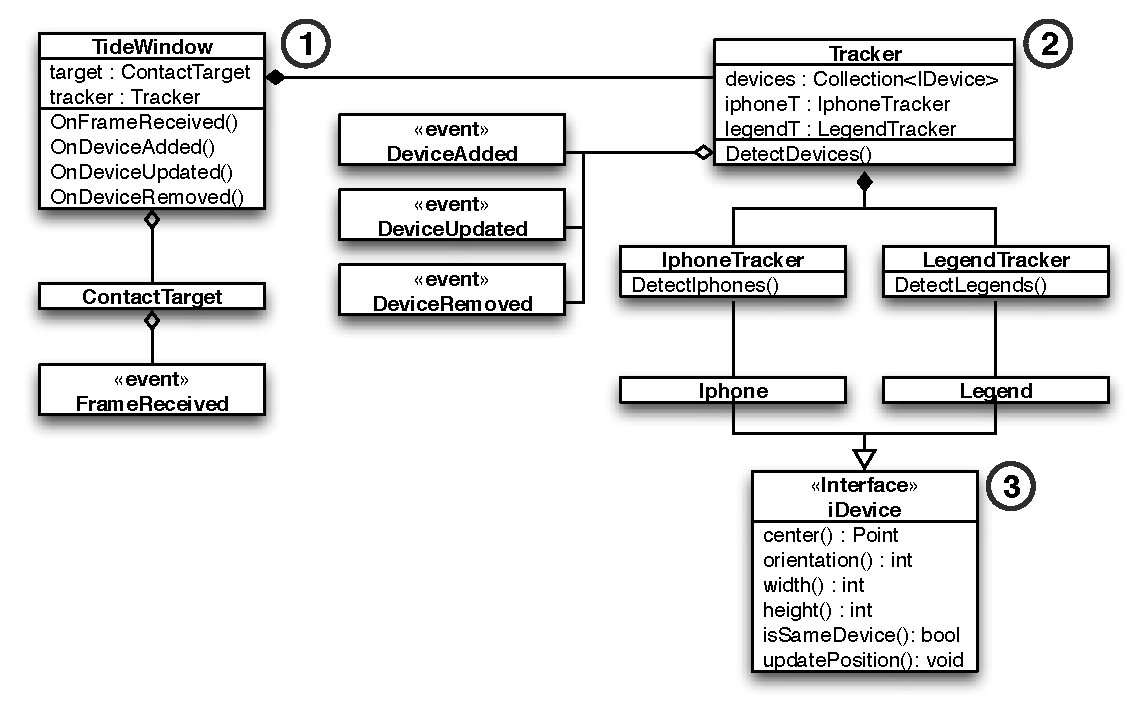
\includegraphics[width=1\textwidth]{images/trackingDiagram}
    \caption{Class diagram of the tracking component.}
    \label{fig:trackingDiagram}
\end{figure}

Figure~\ref{fig:trackingDiagram} shows the implementation that allows TIDE to detect specific smartphones, and track their whereabouts on the surface during application sessions.

The \texttt{TIDEWindow} (\raisebox{.5pt}{\textcircled{\raisebox{-.9pt} {1}}}) is an application-specific instance of a \texttt{SurfaceWindow} control provided by the Surface SDK Presentation layer. 
It represents the main application window, and comprises most of the application logic.
The core layer of the Surface SDK provides the \texttt{ContactTarget} class, which raises the \texttt{FrameReceived} event for each available frame of visual input.

The \texttt{TideWindow} sends screen captures to the \texttt{Tracker} class (\raisebox{.5pt}{\textcircled{\raisebox{-.9pt} {2}}}), that is responsible for processing the images, detecting and tracking the smartphones.
The \texttt{Tracker} keeps track of the devices by using additional tracker classes that are specific to the supported device types.
In the current implementation, the \texttt{IphoneTracker} detects \texttt{Iphone} objects, and the \texttt{LegendTracker} detects \texttt{Legend} objects.
All device types implement the \texttt{IDevice} interface (\raisebox{.5pt}{\textcircled{\raisebox{-.9pt} {3}}}), which provides properties that are used by the main \texttt{Tracker} to keep track of an updated list of current devices.
Upon device apparition, movement or removal, the \texttt{Tracker} raises relevant events, i.e.\ \texttt{DeviceAdded}, \texttt{DeviceUpdated}, \texttt{DeviceRemoved}.
The \texttt{TIDEWindow} listens for such events, and handles them accordingly.

The tracking component provides the application with the means to know when new devices are placed on the table, but also when and where they are moved, and when they are removed entirely.
The initial device detection was used in the evaluated prototype, as a trigger for pairing.

However, the tracking of smartphone devices during the application session was deactivated for the test sessions.
This decision was based on feedback gathered during the prototyping sessions, that pointed towards a lack of usefulness.
Users expressed that they would not want to leave their smartphones on the table where it could be stolen.
Some would not want to drag the device across the table because of possible damage.

%%%%%%%%%%%%%%%%
%% REPLICATION %%
%%%%%%%%%%%%%%%%
\section{Replicated UI}
\label{sec:replicatedui}

% EXPLAIN MAPPING, BUTTONS, DETAILED IMPLEMENTATION?

This section describes and explains the implementation steps that were taken based on the design decisions from section~\ref{sec:design} relating to the replicated UI.

To realize the design decision
\emph{DC-1 The smartphone screen is replicated to the tabletop using a standard desktop sharing protocol}, 
it was decided to use VNC \citep{Richardson:1998:vnc}, a standard system that uses a rendering-based protocol to allow desktop sharing between remote computers.
It works with a network connection between a client and a server, where the client sends input events to the server, which responds by sending a pixel-based copy of its updated screen.
It was chosen for its stability and library availability on many platforms.

%The pairing procedure completes with the VNC client on the tabletop connecting to the VNC server running on the smartphone, and receiving the first image of the remote UI.

On the tabletop, the VNC client is integrated to the Surface application using a \texttt{VncControl} object.
The \texttt{VncControl} is a surface user control that is contained within a \texttt{DeviceControl} object that provides other UI elements, as shown in figure \ref{fig:tideControls}.
The \texttt{DeviceControl} object monitors all contacts, in order to detect the user inputs that are destined to the replicated UI.
This is done by checking if the coordinates of the contact are within the image displayed by the \texttt{VncControl}.
When such a contact is detected, it is forwarded to the \texttt{VncControl} object, that relays it further to the smartphone.

\begin{figure}[htb]
  \centering
    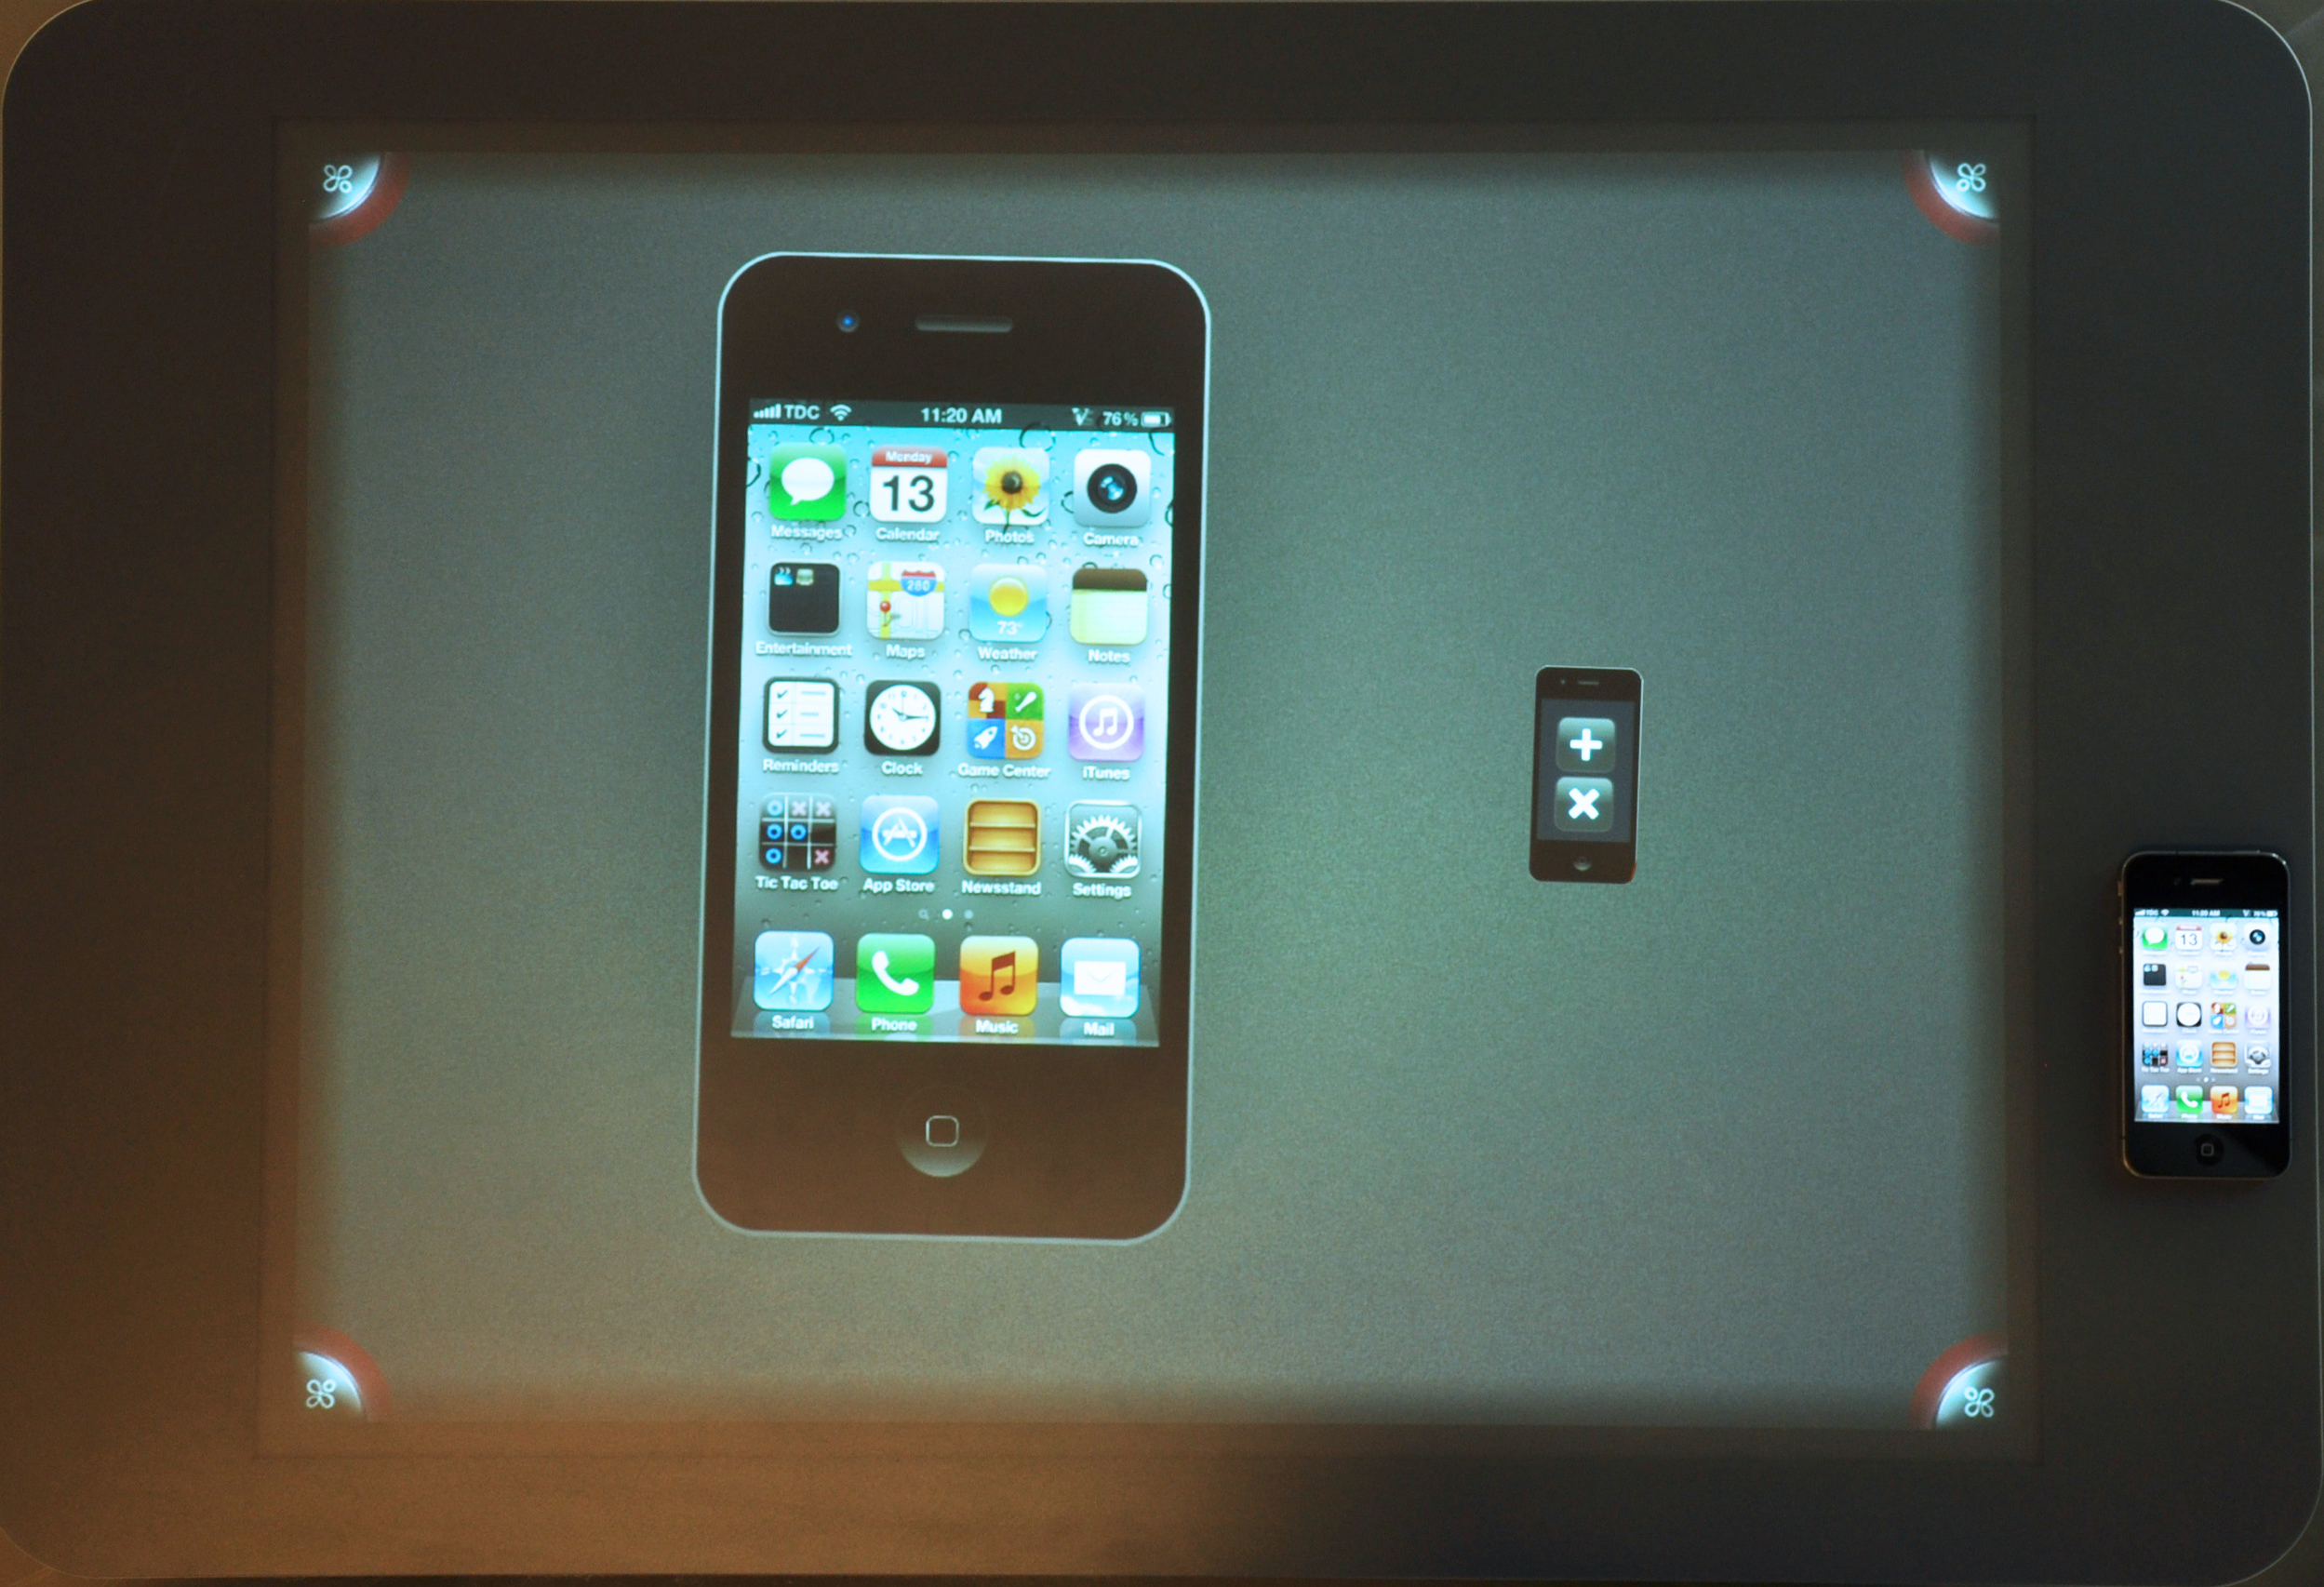
\includegraphics[width=0.7\textwidth]{images/tideControls}
    \caption{TIDE main UI elements.}
    \label{fig:tideControls}
\end{figure}

The \texttt{VncControl} uses the VncSharp library to communicate with the VNC server on the smartphone.
VncSharp provides methods to transmit mouse and keyboard events.
%Mouse events consist of coordinates a contact type (\texttt{ContactDown, ContactUp and ContactChanged}), and they are used for all touch inputs on the replicated UI.
The server responds with an updated image of the smartphone's screen, that the \texttt{VncControl} displays on the tabletop.

On the smartphones, the VNC server relies currently on third-party applications; Veency on iOS, and Droid VNC Server on Android.
The reason for this was to allow the easy integration of devices running on different platforms.



%%%%%%%%%%%%%%
%% SURFACE %%
%%%%%%%%%%%%%%
\section{Surface UI}
\label{sec:surfaceui}

This section describes and explains the implementation steps that were taken based on the design decisions in section~\ref{sec:design} relating to the surface UI.
To realize the design decisions DD-1 to DD-6 (see p.~\pageref{DD}), TIDE is implemented using the Surface SDK, which is itself based on WPF (Windows Presentation Foundations).

The elements from figure~\ref{fig:tideControls} are described below in figure~\ref{fig:surfaceDiagram}, which is a class diagram of the TIDE surface UI implementation.

As mentioned for the tracking component, the \texttt{TideWindow} (\raisebox{.5pt}{\textcircled{\raisebox{-.9pt} {1}}}) is the main application window.
It contains all other UI elements and is responsible for most of the application logic.
The \texttt{DeviceControl} (\raisebox{.5pt}{\textcircled{\raisebox{-.9pt} {2}}}) contains the replicated UI of a connected smartphone, and provides the main surface UI elements to the user.
The \texttt{MinimizedControl} (\raisebox{.5pt}{\textcircled{\raisebox{-.9pt} {3}}}) is the minimized version of the \texttt{DeviceControl}.

\begin{figure}[htb]
  \centering
    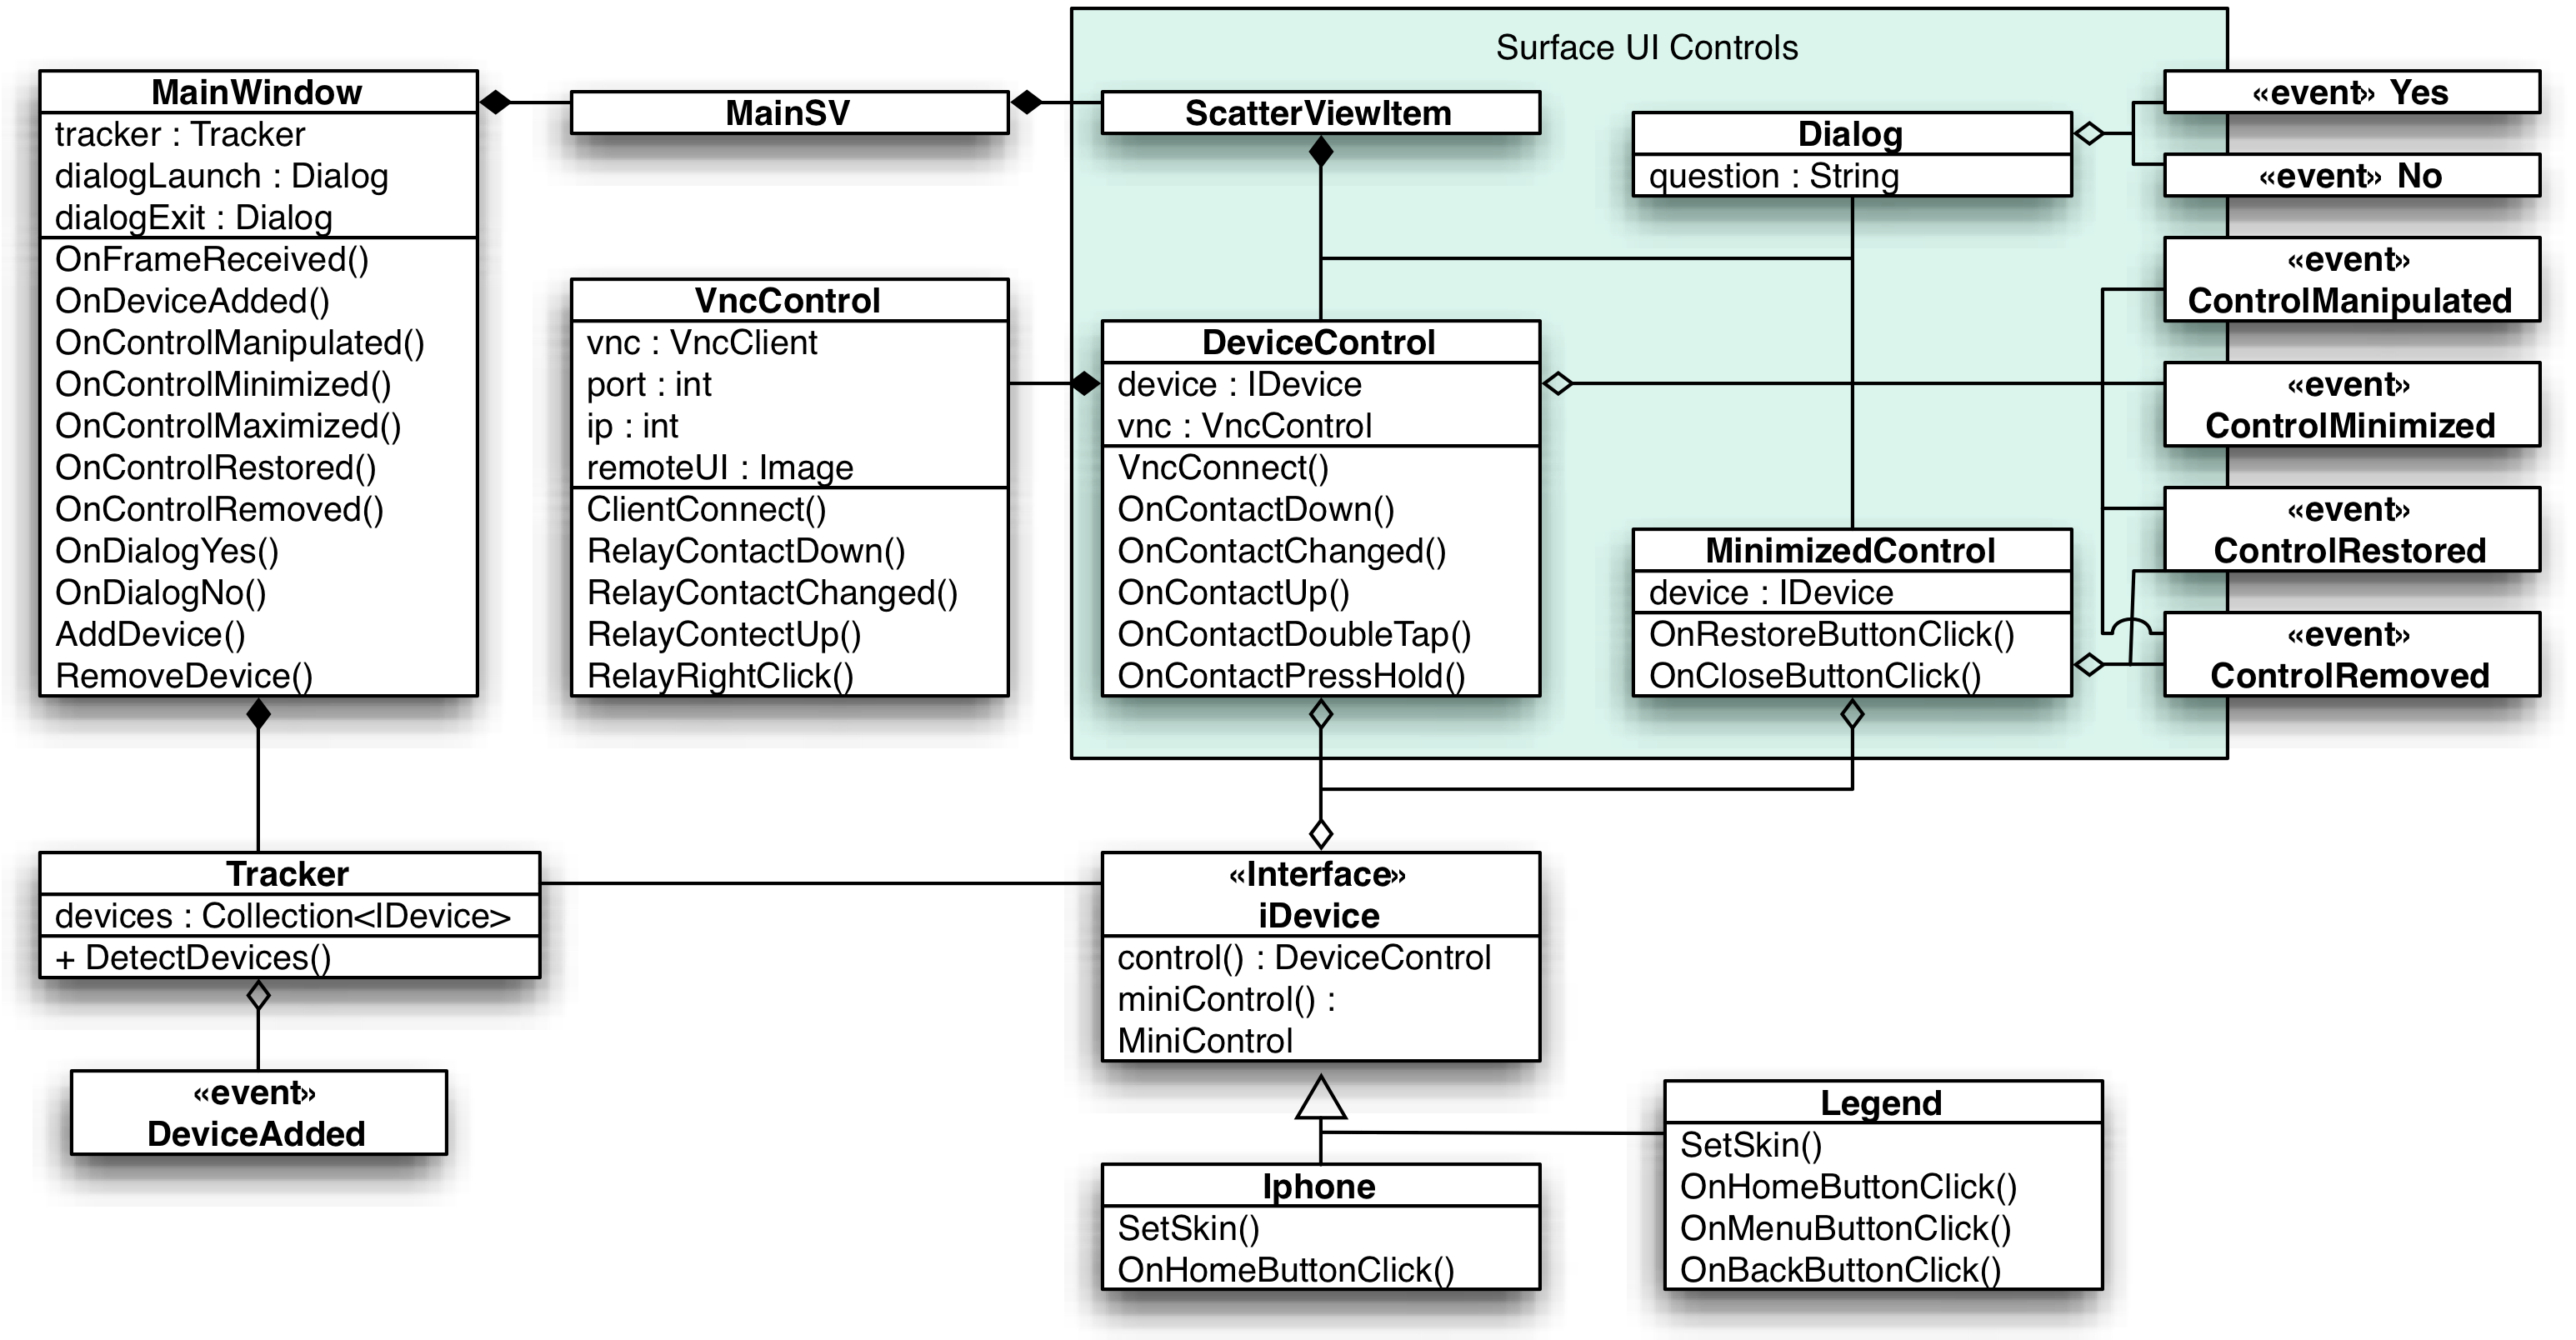
\includegraphics[width=1\textwidth]{images/surfaceDiagram}
    \caption{Class diagram of the surface UI.}
    \label{fig:surfaceDiagram}
\end{figure}

The implementation of the surface UI is based on the Presentation layer of the Surface SDK.
To realize the design decision
\emph{DD-2 The replicated UI can be manipulated by using touch-based gestures on the surface UI},
TIDE uses a \texttt{ScatterView} object called \texttt{MainScatterView}.
The \texttt{ScatterView} control displays UI elements that can be manipulated, by wrapping them inside \texttt{ScatterViewItem} objects.
The \texttt{ScatterViewItem} class provides manipulation capabilities to the surface controls, that include move, rotate and resize with one or several fingers.
However, some of these capabilities are deactivated for specific controls, such as the \texttt{MinimizedControl}, which cannot be resized.

Each virtual device consists of three objects; a \texttt{Device} implementing the \texttt{IDevice} interface, and two surface controls; the \texttt{DeviceControl} and \texttt{MinimizedControl} objects.

Upon creation, the \texttt{DeviceControl} object gets specific visualization features from its \texttt{Device}.
An example being that an \texttt{iPhone} object provides a \texttt{SetSkin()} method to show the appropriate visualization, and \texttt{OnHomebuttonClick()} that implements the effect of the home button, specific to the iPhone.

The \texttt{DeviceControl} monitors all its touch inputs, and reacts differently depending on the location.
If the input is within the \texttt{VncControl} image, it is forwarded to the replicated UI.
Otherwise, the input is interpreted as a manipulation on the containing \texttt{ScatterViewItem} object.
The features that are activated by a double tap, press and hold, and whole hand tap are also implemented within the \texttt{DeviceControl} class.

%The \texttt{DeviceControl} object is displayed on the \texttt{TideWindow}, it can be freely moved, rotated and resized.
%However, it monitors all touch inputs, and forwards to the \texttt{VncControl} all inputs that are destined to the replicated UI, i.e.\ whose coordinates are within the \texttt{remoteUI} image displayed by the \texttt{VncControl}.

When a \texttt{DeviceControl} is minimized, it raises an event that is handled by the \texttt{TideWindow}, causing the \texttt{DeviceControl} to be hidden, and the \texttt{MinimizedControl} to be shown.
Similar events are used to handle restoring and closing controls.

An event called \texttt{ControlManipulated} is used by the \texttt{TideWindow} to monitor the position of the \texttt{DeviceControl} and activate the features that depend on position, size or rotation; such as the minimization when the control is dragged to an edge.

Lastly, \texttt{Dialog} objects are used to obtain explicit user confirmation when establishing the connection and when disconnecting the device.
They are surface controls that are wrapped in \texttt{ScatterViewItem} objects, and their manipulation capabilities are deactivated.



